\documentclass[a4paper,12pt]{article}
\usepackage[utf8]{inputenc}
\usepackage[spanish]{babel}
\usepackage{graphicx}
\usepackage{float}

%opening
\title{Tarea No. 1. JDBC }
\author{Barrera Pérez Carlos Tonatihu \\ Profesor: José Asunción Enríquez Zárate \\ Web Application Development \\ Grupo: 3CM9 }

\begin{document}

\maketitle
\newpage
\tableofcontents

\newpage
\section{Introducción}
Este trabajo es una investigación sobre la conectividad a bases de datos de Java.

Java Database Connectivity o JDBC es una interfaz de acceso a bases de datos estándar SQL que proporciona un acceso uniforme a una gran variedad de bases de datos relacionales. También proporciona una base común para la construcción de herramientas y utilidades de alto nivel. Todo esto orientado al lenguaje de programación Java.

\newpage
\section{Desarrollo}
\subsection{¿Qué es?}
JDBC es el API para la ejecucion de sentencias SQL. Consiste en un conjunto de clases e interfaces escritas en el lenguaje de programación Java. JDBC suministra una API estándar para los desarrolladores y hace posible escribir aplicaciones de base de datos usando un API puro de Java \cite{PAGINA}.

Usando JDBC es fácil enviar sentencias SQL virtualmente a cualquier sistema de base de datos. En otras palabras, con el API JDBC, no es necesario escribir un programa que acceda a una base de datos Sybase, otro para acceder a Oracle y otro para acceder a Informix. Un único programa escrito usando el API JDBC y el programa será capaz de enviar sentencias SQLa la base de datos apropiada. Y, con una aplicación escrita en el lenguaje de programación Java, tampoco es necesario escribir diferentes aplicaciones para ejecutar en diferentes plataformas. La combinación de Java y JDBC permite al programador escribir una sola vez y ejecutarlo en cualquier entorno.

\begin{figure}[H]
\begin{center}
 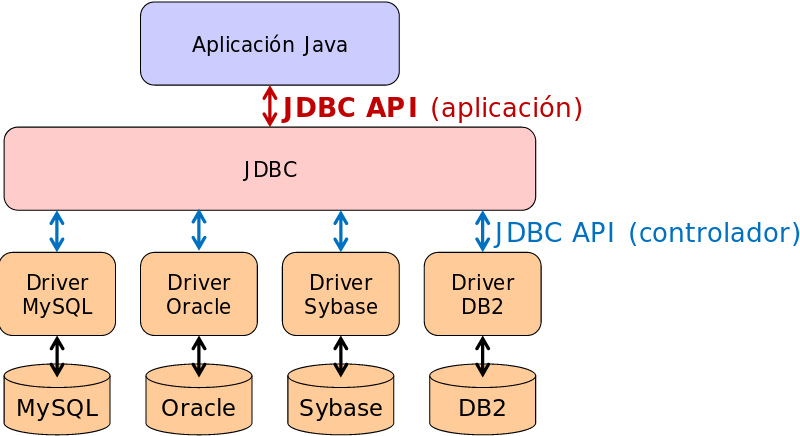
\includegraphics[width=12cm]{estructura.png}
 % estructura.png: 800x436 px, 96dpi, 21.16x11.53 cm, bb=0 0 600 327
 \caption{Estructura de JDBC}
 \label{fig:estructura}
\end{center}
\end{figure}



\subsection{¿Qué hace?}
JDBC hace posible estas tres cosas:
\begin{enumerate}
 \item Establece una conexión con la base de datos.
 \item Envia sentencias SQL.
 \item Procesa los resultados.
\end{enumerate}

Para realizar esto se utiliza el paquete java.sql y javax.sql los cuales ofrecen \cite{PDF}.

\begin{itemize}
 \item Uso de controladores de las bases de datos.
 \begin{itemize}
  \item Clase DriverManager. Permite establecer y gestionar conexiones a las bases de datos.
  \item Clase SQLPermission. Proporciona los permisos para poder usar el DriverManager a código en ejecución dentro de un Security Manager.
  \item Interfaz Driver. Metodos para registrar y conectar controladores basados en tecnología JDBC.
  \item Clase DriverPropertyInfo. Propiedades de un controlador.
 \end{itemize}
 
 \item Excepciones
 \begin{itemize}
  \item SQLException
  \item SQLWarning
 \end{itemize}
 
 \item Envío de instrucciones SQL a la BD
 \begin{itemize}
  \item Connection. Métodos para crear instrucciones y para gestionar conexiones y sus propiedades.
  \item Statement. Permite enviar instrucciones a la BD.
  \item PreparedStatement. Permite usar instrucciones preparadas o SQL básicas.
  \item CallableStatement.Llamada a procedimientos almacenados en la BD.
  \item Savepoint. Puntos de recuperación en una transacción.
 \end{itemize}
 
 \item Recuperación de los resultados a la consulta a la base de datos.
 \begin{enumerate}
  \item ResultSet. Conjunto de resultados que se devuelven de una query.
  \item ResultSetMetaData. Información sobre las columnas del objeto ResultSet.
 \end{enumerate}

\end{itemize}

\subsection{¿Cómo se hace?}
La secuencia para poder trabajar con JDBC es la siguiente:
\begin{enumerate}
 \item Establecer la conexión con la base de datos
 \begin{itemize}
  \item Cargar los controladores (Solo en versiones java inferiores a la 6).
  \item Establecer la conexión.
 \end{itemize}
 
 \item Crear un objeto Statement para hacer petición a la BD.
 \begin{itemize}
  \item Asociar una sentencia SQL al objeto Statement.
  \item Proporcionar valores de los parámetros.
  \item Ejecutar el objeto Statement
 \end{itemize}
 
 \item Procesar los resultados.
 \item Liberar recursos (cerrar la conexión).

\end{enumerate}

\subsection{Tipos de drivers}
Los drivers JDBC drivers son adaptadores del lado del cliente (instalados en la máquina cliente, no en el servidor) que convierten la petición proveniente del programa JAVA a un protocolo que el SGBD pueda entender.

\begin{enumerate}
 \item Driver JDBC Tipo 1 (también llamado Puente JDBC-ODBC) convierte el método JDBC a una llamada a una función ODBC. Utiliza los drivers ODBC para conectar con la base de datos.
 \item Driver JDBC Tipo 2 (también llamado driver API-Nativo) convierte el método JDBC a llamadas nativas de la API de la base de datos. Es más rápido que el puente JDBC-ODBC pero se necesita instalar la librería cliente de la base de datos en la máquina cliente y el driver es dependiente de la plataforma.
 \item  Driver JDBC Tipo 3. Hace uso de un Middleware entre el JDBC y el SGBD.
 \item Driver JDBC Tipo 4 (también llamado Driver Java Puro directo a la base de datos). Es independiente a la plataforma.
\end{enumerate}

La elección de que driver usar se puede hacer siguiendo los siguientes criterios.
\begin{enumerate}
 \item Si se accede a un tipo de base de datos se recomienda el tipo 4.
 \item Si se accede a multiples tipos de bases de datos al mismo tiempo el driver 3 es el mejor.
 \item Si el driver tres o cuatro no están disponibles se debe utilizar el tipo dos.
 \item El tipo uno sólo se debe de utilizar en pruebas y desarrollo.
\end{enumerate}

\section{Conclusiones}
El uso de JDBC en el desarrollo de aplicaciones que se comuniquen con bases de datos es fundamental ya que de no utilizarlo el desarrollo seria demasiado tedioso y repetitivo ya que se tendria que estar trabajando desde cero la conexión a las diferentes bases de datos que existen. Y no se puede simplemente el optar por no utilizar bases de datos ya que en la actualidad su uso es fundamental en el desarrollo de aplicaciones robustas y que puedan satisfacer las necesidades de los usuarios.

\bibliographystyle{ieeetr}
\bibliography{referencias}

\end{document}
